\section{Konzept}

\subsection{Systemarchitektur}

    \subsubsection*{Überblick}

    Für das Cloudbasierte Praxisruf System sehen wir fünf Komponenten vor: 

    \begin{itemize}
        \item Messaging Service
        \item Cloud Service
        \item Mobile Client
        \item Admin UI
        \item VOIP Mediator
    \end{itemize}


    \begin{figure}[H]
    \centering
    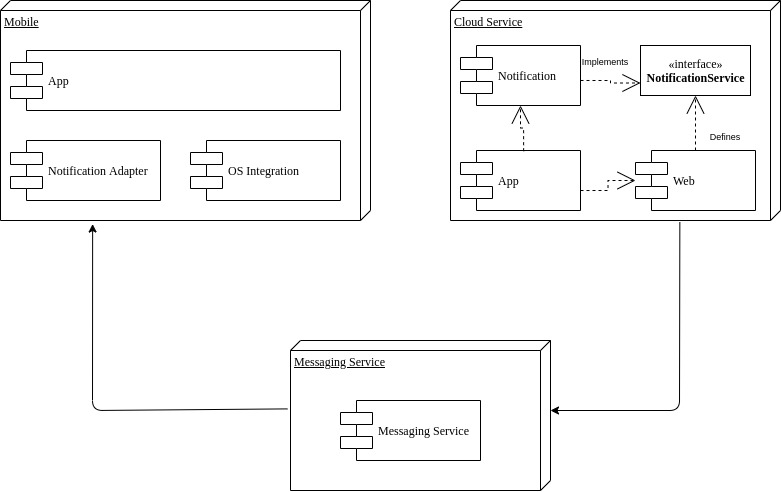
\includegraphics[width=\linewidth]{IP5_POC_Cloud_Architecture.jpg}
    \end{figure}


    \subsubsection*{Mobile Client}

        \begin{itemize}
            \item Der Mobile Client implementiert die Anbindung an den Messaging Service. 
            \item Als Reaktion auf eine Notification wird eine Rückmeldung im UI angezeigt. 
            \item Als Reaktion auf eine Notification wird eine OS Push Notifikation gesendet. 
            Das UI bietet einen Button der eine Anfrage an die REST Schnittstelle im Cloud Service sendet. 
        \end{itemize}


    \subsubsection*{Cloud Service}

        \begin{itemize}
            \item Responsibilities (Notification and Configuration)
            \item Microservice Granularity
        \end{itemize}


    \subsubsection*{Messaging Service}

        \begin{itemize}
            \item Dies wird ein externer Service den wir in die Applikationen einbinden. Standard hierfür ist Firebase Notifications. 
            \item Der Messaging Service nimmt Notifikationen vom Cloud Service entgegen und gibt diese an den Mobile Client wieder. 
            \item Dafür müssen auf beiden Seiten Komponenten eingebaut werden, die mit dem Messaging Service kommunizieren.
        \end{itemize}


\subsection{Mobile Client}
    \subsubsection{Architektur}
    \subsubsection{User Interface}

\subsection{Cloud Service}
    \subsubsection{Architektur}
    \subsubsection{Domänenmodell}
    \subsubsection{Laufzeitmodell}

\subsection{Admin UI}

\subsection{Proof Of Concept}
\subsubsection*{Anforderungen}

\begin{itemize}
    \item Als <Sender Rolle> möchte ich Notifikationen versenden können. 
    \item Als <Empfänger Rolle> möchte ich Notifikationen in der Applikation sehen, wenn die Applikation geöffnet ist.  
    \item Als <Empfänger Rolle> möchte ich Notifikationen über das OS erhalten, wenn die Applikation minimiert ist. 
\end{itemize}

\subsubsection*{Restriktionen}

\begin{itemize}
    \item Nur 1 Client. 
    \item Nur 1 fixe Notifikation. Keine Types. 
    \item Notifikation wird vom Client gesendet und vom selben Client empfangen. 
    \item Keine Authentication oder Authorization. 
  
\end{itemize}


